%----------------------------------------------------------------------------
\chapter{Background and related work}
\label{chap:background}
%----------------------------------------------------------------------------

%----------------------------------------------------------------------------
\section{Graph neural networks}
\label{sec:gnn}
%----------------------------------------------------------------------------

\subsection{Text-attributed graphs and homophily}
\label{sec:tag}

For a graph $G = (V, E)$, the neighbourhood of a node $v$ is $\mathcal{N}(v) = \{u \in V : (u, v) \in E\}$; in a directed graph these are the nodes with an edge pointing into $v$. Each node carries a feature vector $\mathbf{x}_v \in \mathbb{R}^d$. A text-attributed graph (TAG) is a graph whose nodes also carry a piece of text $t_v$, for example the title and abstract of a paper in a citation graph. The node features of a TAG can be computed from this text, for instance as an embedding of $t_v$ produced by a text encoder.

Many real-world graphs are homophilous: connected nodes tend to have related content, that is, they often belong to the same class or have similar features~\cite{zhu2020beyond}. A citation graph is an example, since papers tend to cite papers from the same research area~\cite{zhu2020beyond}. Many neighbourhood-aggregation architectures work well when connected nodes have similar features, but generalise poorly to heterophilous graphs, in which linked nodes tend to be dissimilar~\cite{zhu2020beyond}.

\subsection{Message passing}
\label{sec:message-passing}

Gilmer \etal~\cite{gilmer2017neural} reformulated a number of earlier graph neural networks into a single framework, which they call message passing neural networks (MPNNs). The framework is defined on an undirected graph $G$ whose nodes carry feature vectors $\mathbf{x}_v$, and it extends directly to directed graphs~\cite{gilmer2017neural}. The framework also allows features on the edges; they are omitted here, because the graphs in this thesis have none.

The message passing phase of an MPNN runs for $T$ steps. Every node $v$ keeps a hidden state $\mathbf{h}_v^{(t)}$, initialised with its features, $\mathbf{h}_v^{(0)} = \mathbf{x}_v$. At each step, a message function $M_t$ computes a message from every neighbour, the messages are summed, and a vertex update function $U_t$ combines the result with the node's current state:
\begin{align}
  \mathbf{m}_v^{(t+1)} &= \sum_{w \in \mathcal{N}(v)} M_t\big(\mathbf{h}_v^{(t)}, \mathbf{h}_w^{(t)}\big), \label{eq:mp-message} \\
  \mathbf{h}_v^{(t+1)} &= U_t\big(\mathbf{h}_v^{(t)}, \mathbf{m}_v^{(t+1)}\big). \label{eq:mp-update}
\end{align}
Gilmer \etal follow this phase with a readout phase that computes an output for the whole graph; for tasks with a target at each node, the final node states $\mathbf{h}_v^{(T)}$ themselves serve as the output~\cite{gilmer2017neural}.

Since each step brings in information from one more hop, the state $\mathbf{h}_v^{(T)}$ can receive information from nodes up to $T$ hops away, following the direction in which messages flow. \autoref{fig:message-passing} illustrates this on a citation neighbourhood. Repeated neighbourhood aggregation, however, can make node representations increasingly similar, a phenomenon known as over-smoothing~\cite{li2018deeper}.

\begin{figure}[!ht]
  \centering
  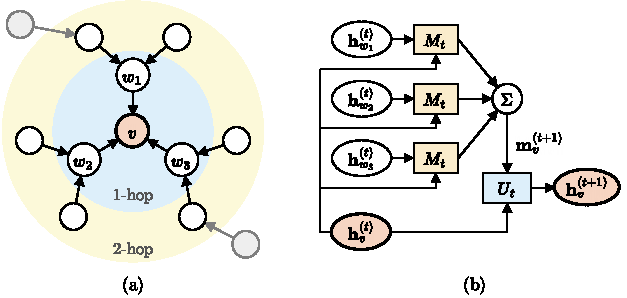
\includegraphics{../diagrams/figures/background/message_passing.pdf}
  \caption{(a)~The neighbourhood of a target paper $v$ in a citation graph; messages flow along the edges towards $v$. After $T=1$ step, $\mathbf{h}_v^{(T)}$ can contain information from the 1-hop neighbourhood (inner shading), and after $T=2$ steps from the 2-hop neighbourhood (outer shading); the grey nodes lie further away. (b)~One message passing step at $v$, as in \eqref{eq:mp-message}--\eqref{eq:mp-update}: $M_t$ computes a message from the state of each neighbour and $\mathbf{h}_v^{(t)}$, the messages are summed, and $U_t$ combines the sum with the current state of $v$.}
  \label{fig:message-passing}
\end{figure}

\subsection{GraphSAGE}
\label{sec:graphsage}

Many earlier methods for node embedding train a separate vector for every node. Such methods are inherently transductive: they do not naturally generalise to nodes that were not seen during training~\cite{hamilton2017inductive}. GraphSAGE is an inductive framework instead: rather than an embedding for each node, it learns a function that generates the embedding of a node by sampling and aggregating features from its local neighbourhood, so the same function can also embed nodes that are new~\cite{hamilton2017inductive}.

In the following, $\mathbf{h}_v \in \mathbb{R}^d$ denotes the state of node $v$ at the input of a layer and $\mathbf{h}'_v \in \mathbb{R}^{d'}$ its state at the output. A GraphSAGE layer first aggregates the states of the neighbours into a single vector, then concatenates it with the node's own state and applies a learned matrix $\mathbf{W} \in \mathbb{R}^{d' \times 2d}$ and a nonlinearity $\sigma$~\cite{hamilton2017inductive}:
\begin{align}
  \mathbf{h}_{\mathcal{N}(v)} &= \mathrm{AGGREGATE}\big(\{\mathbf{h}_w : w \in \mathcal{N}(v)\}\big), \label{eq:sage-aggregate} \\
  \mathbf{h}'_v &= \sigma\big(\mathbf{W} \, [\mathbf{h}_v \,\Vert\, \mathbf{h}_{\mathcal{N}(v)}]\big), \label{eq:sage-update}
\end{align}
where $\Vert$ denotes concatenation. The output is then normalised to unit $L_2$ norm. Keeping the node's own state apart from the aggregated neighbour states is a simple form of skip connection~\cite{hamilton2017inductive}. Splitting $\mathbf{W}$ into its left and right halves, $\mathbf{W} = [\mathbf{W}_1 \,\Vert\, \mathbf{W}_2]$, shows that the layer applies separate weights to the node itself and to its neighbours:
\begin{align}
  \mathbf{W} \, [\mathbf{h}_v \,\Vert\, \mathbf{h}_{\mathcal{N}(v)}] = \mathbf{W}_1 \mathbf{h}_v + \mathbf{W}_2 \mathbf{h}_{\mathcal{N}(v)}.
  \label{eq:sage-split}
\end{align}
In terms of the message passing framework, the message from a neighbour is its state itself, the sum in~\eqref{eq:mp-message} is replaced by the aggregator, and~\eqref{eq:sage-update} is the update function.

Since the neighbours of a node have no natural ordering, the aggregator should be symmetric, that is, invariant to permutations of its inputs~\cite{hamilton2017inductive}. The mean aggregator takes the element-wise mean of the neighbour states:
\begin{align}
  \mathbf{h}_{\mathcal{N}(v)} = \frac{1}{|\mathcal{N}(v)|} \sum_{w \in \mathcal{N}(v)} \mathbf{h}_w.
  \label{eq:sage-mean}
\end{align}
Finally, the original GraphSAGE procedure samples a fixed-size set of neighbours uniformly at each layer, to keep the computational cost of each training batch fixed~\cite{hamilton2017inductive}.

\subsection{Graph attention: GATv2}
\label{sec:gatv2}

Unlike the mean aggregator, GATv2~\cite{brody2022attentive} computes a weighted average of the neighbour states, with attention weights computed from the states themselves. A scoring function assigns every neighbour $w$ of $v$ a score that indicates the importance of the features of $w$ to $v$. The function applies a learned matrix to the concatenated states, then a nonlinearity, then a learned vector $\mathbf{a}$, which in effect computes the score of every pair with a small multilayer perceptron~\cite{brody2022attentive}:
\begin{align}
  e(\mathbf{h}_v, \mathbf{h}_w) = \mathbf{a}^\top \mathrm{LeakyReLU}\big(\mathbf{W}_1 \mathbf{h}_v + \mathbf{W}_2 \mathbf{h}_w\big),
  \label{eq:gatv2-score}
\end{align}
where $\mathbf{W}_1, \mathbf{W}_2 \in \mathbb{R}^{d' \times d}$ are the left and right halves of the matrix applied to $[\mathbf{h}_v \,\Vert\, \mathbf{h}_w]$, and $\mathbf{a} \in \mathbb{R}^{d'}$. LeakyReLU is applied element-wise:
\[
  \mathrm{LeakyReLU}(x) =
  \begin{cases}
    x, & x \geq 0, \\
    \lambda x, & x < 0,
  \end{cases}
  \qquad 0 < \lambda < 1.
\]
The scores are normalised with a softmax over the neighbours of $v$ and $v$ itself~\cite{velickovic2018graph}, and the new state is the weighted average of the transformed states, followed by a nonlinearity:
\begin{align}
  \alpha_{vw} &= \mathrm{softmax}_{w \in \mathcal{N}(v) \cup \{v\}}\big(e(\mathbf{h}_v, \mathbf{h}_w)\big), \label{eq:gatv2-softmax} \\
  \mathbf{h}'_v &= \sigma\Big(\sum_{w \in \mathcal{N}(v) \cup \{v\}} \alpha_{vw} \mathbf{W}_2 \mathbf{h}_w\Big). \label{eq:gatv2-output}
\end{align}
In terms of the message passing framework, the message from $w$ is $\alpha_{vw}\mathbf{W}_2\mathbf{h}_w$, with the difference that $\alpha_{vw}$ depends on all neighbours of $v$ through the softmax normalisation.

In the original graph attention network (GAT)~\cite{velickovic2018graph}, the relative ranking of candidate neighbours is independent of the query node~\cite{brody2022attentive}. GATv2 changes the order of the scoring operations so that this ranking can depend on the query node~\cite{brody2022attentive}.

%----------------------------------------------------------------------------
\section{Large language models}
\label{sec:llm}
%----------------------------------------------------------------------------

\subsection{The Transformer and self-attention}
\label{sec:transformer}

Large language models (LLMs) are built on the Transformer~\cite{vaswani2017attention}. The input text is split into tokens, and each token is mapped to an embedding vector of dimension $d_{\text{model}}$. The original Transformer has an encoder--decoder structure, and both the encoder and the decoder are stacks of layers with the same structure. An encoder layer consists of a multi-head self-attention block and a position-wise feed-forward network; a decoder layer adds a third block, which attends to the output of the encoder. Each block is wrapped in a residual connection and layer normalisation~\cite{vaswani2017attention}. Most modern LLMs, including the Qwen3 model used in this thesis, use only the decoder stack, without the encoder and therefore without the third block: each layer consists of masked multi-head self-attention and a feed-forward network (\autoref{fig:transformer}a).

\begin{figure}[!ht]
  \centering
  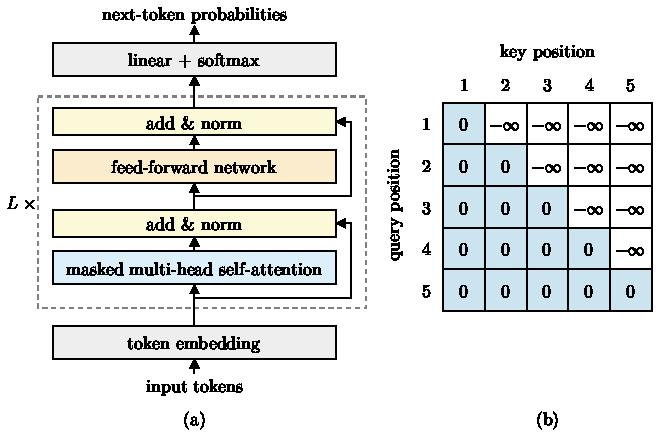
\includegraphics{../diagrams/figures/background/transformer_causal_mask.pdf}
  \caption{(a)~A schematic decoder-only Transformer; the dashed block is repeated $L$ times. (b)~The causal mask for five positions, added to the attention scores before the softmax.}
  \label{fig:transformer}
\end{figure}

An attention function maps a query and a set of key--value pairs to an output. The output is a weighted sum of the values, where the weight of each value is computed from the query and the corresponding key~\cite{vaswani2017attention}. In self-attention, the queries, keys and values all come from the same sequence. With the hidden states of the positions stacked as the rows of a matrix $\mathbf{X}$, they are $\mathbf{Q} = \mathbf{X}\mathbf{W}^Q$, $\mathbf{K} = \mathbf{X}\mathbf{W}^K$ and $\mathbf{V} = \mathbf{X}\mathbf{W}^V$, where $\mathbf{W}^Q, \mathbf{W}^K \in \mathbb{R}^{d_{\text{model}} \times d_k}$ and $\mathbf{W}^V \in \mathbb{R}^{d_{\text{model}} \times d_v}$ are learned. The Transformer uses scaled dot-product attention~\cite{vaswani2017attention}:
\begin{align}
  \mathrm{Attention}(\mathbf{Q}, \mathbf{K}, \mathbf{V}) = \mathrm{softmax}\Big(\frac{\mathbf{Q}\mathbf{K}^\top}{\sqrt{d_k}}\Big)\mathbf{V}.
  \label{eq:attention}
\end{align}
Here $d_k$ is the dimension of the queries and keys, $d_v$ that of the values, and the softmax is applied to each row separately. The scaling by $1/\sqrt{d_k}$ keeps the dot products from growing large in magnitude, which would push the softmax into regions with extremely small gradients~\cite{vaswani2017attention}. Query--key similarities determine the attention weights, which are used to combine the value vectors.

Instead of a single attention function, the Transformer uses multi-head attention: $H$ heads, each with its own projection matrices, compute attention in parallel, and their outputs are concatenated and projected once more. This allows the model to attend jointly to information from different representation subspaces at different positions~\cite{vaswani2017attention}.

In a decoder, a position must not see the positions that follow it, so that the model stays autoregressive: each position may attend only to itself and to the positions before it. This is implemented inside the attention function by setting the scores of all forbidden query--key pairs to $-\infty$ before the softmax, which gives them zero weight~\cite{vaswani2017attention}. Attending to the current position does not reveal the answer, because the representation at a position is used to predict the next token~\cite{vaswani2017attention}. \autoref{fig:transformer}b shows the resulting mask.

\subsection{Language modelling and decoding}
\label{sec:decoding}

Given a context $c$, for example a prompt, an autoregressive language model assigns a probability to a token sequence $y_1, \dots, y_N$:
\begin{align}
  p(y_{1:N} \mid c) = \prod_{n=1}^{N} p(y_n \mid c, y_{<n}).
  \label{eq:lm-factorisation}
\end{align}
The sequence is therefore generated one token at a time: the model predicts a probability distribution over the next token, conditioned on the context and on the tokens before it~\cite{vaswani2017attention}. The model is trained by minimising the next-token cross-entropy over the target tokens, that is, their negative log-likelihood:
\begin{align}
  \mathcal{L} = -\sum_{n=1}^{N} \log p(y_n \mid c, y_{<n}).
  \label{eq:lm-loss}
\end{align}
During training, each prediction is conditioned on the preceding ground-truth tokens, a procedure called teacher forcing. All target-token losses can therefore be computed in parallel in a single forward pass, with causal masking preventing access to future tokens.

At generation time, a decoding strategy chooses each token from the predicted distribution. Greedy decoding always takes the most probable token, $\hat{y}_n = \argmax_{y} p(y \mid c, \hat{y}_{<n})$, so it is deterministic; sampling-based strategies draw the token at random from the distribution instead.

\subsection{The key--value cache and grouped-query attention}
\label{sec:kv-cache}

When a sequence is generated one token at a time, the keys and values of the earlier positions do not change as new tokens are appended, because the causal mask stops the earlier positions from attending to them. It is therefore common practice to store the keys and values of all earlier positions in every layer, in what is called the key--value (KV) cache, and to reuse them. Each new token only computes its own query, key and value, adds its key and value to the cache, and attends to all cached keys and values. The attention computation can also incorporate additional learned key and value vectors.

Grouped-query attention (GQA) divides the query heads into groups, each of which shares a single key head and value head~\cite{ainslie2023gqa}. Compared with standard multi-head attention, this reduces the number of keys and values that are stored and read at every decoding step~\cite{ainslie2023gqa}. The number of key--value heads, not the number of query heads, therefore sets how many heads the cached key and value tensors have, and so how many heads any additional key and value vectors need.

\subsection{Positional information}
\label{sec:positional}

Attention by itself has no notion of the order of the positions, so information about position has to be injected~\cite{vaswani2017attention}. Rotary position embedding (RoPE)~\cite{su2024roformer} encodes the absolute position by multiplying the query and the key with a rotation matrix whose angle depends on the position. It is derived from the requirement that the inner product of a query at position $m$ and a key at position $n$ depends on their positions only through the difference $m - n$:
\begin{align}
  \big\langle f_q(\mathbf{x}_m, m), f_k(\mathbf{x}_n, n) \big\rangle = g(\mathbf{x}_m, \mathbf{x}_n, m - n),
  \label{eq:rope}
\end{align}
where $f_q$ and $f_k$ compute the query and the key from the embedding $\mathbf{x}_m$ of the token at position $m$ and from its position~\cite{su2024roformer}. For fixed query and key vectors, the positional dependence introduced by RoPE is therefore determined by their relative displacement~\cite{su2024roformer}.


%----------------------------------------------------------------------------
\section{Soft prompting}
\label{sec:soft-prompting}
%----------------------------------------------------------------------------

\subsection{Hard and soft prompts}
\label{sec:soft-prompts}

A language model can be given a task through a textual instruction, such as ``Summarise the following document.'' This is a hard prompt: text that is tokenised and passed through the embedding layer of the model like any other input. Soft prompting instead introduces trainable continuous vectors, whose values are optimised directly by backpropagation rather than selected from the vocabulary of the model, while the weights of the language model stay fixed~\cite{lester2021power}. The vectors do not have to correspond to the embedding of any vocabulary token, and a soft prompt can be used together with ordinary text: the model reads the soft prompt followed by the embedded input~\cite{lester2021power}.

\subsection{Prompt tuning}
\label{sec:prompt-tuning}

Prompt tuning~\cite{lester2021power} places the soft prompt at the input of the model. The soft prompt is a learned matrix $\mathbf{P}_e \in \mathbb{R}^{M \times d_{\text{model}}}$ of $M$ vectors, which is concatenated with the embeddings of the input tokens; the resulting sequence flows through the model as normal, and only $\mathbf{P}_e$ is updated during training~\cite{lester2021power}. Prompt tuning therefore learns $M d_{\text{model}}$ parameters, and the soft prompt influences the deeper layers only through the frozen network, which gives it a relatively indirect impact on the predictions~\cite{liu2022ptuning}. Experiments with T5 on the SuperGLUE benchmark showed that prompt tuning became more effective as model size increased. For the largest models tested, its performance approached that of full fine-tuning, while updating only the prompt parameters~\cite{lester2021power}.

\subsection{Prefix tuning}
\label{sec:prefix-tuning}

Prefix tuning~\cite{li2021prefix} supplies learned key and value vectors to the attention mechanism at every Transformer layer, rather than introducing learned embeddings only at the input (\autoref{fig:prompt-prefix}). The language model stays frozen, and only these vectors are trained~\cite{li2021prefix}. The subsequent tokens attend to the $M$ prefix positions as if they were ``virtual tokens'', but the activations at these positions are free parameters rather than being computed by the model from a token~\cite{li2021prefix}. For one attention head of layer $\ell$, with the causal mask omitted for clarity, prefix tuning extends the keys and values with learned matrices $\mathbf{P}^K_\ell \in \mathbb{R}^{M \times d_k}$ and $\mathbf{P}^V_\ell \in \mathbb{R}^{M \times d_v}$:
\begin{align}
  \mathrm{Attention}\big(\mathbf{Q}, [\mathbf{P}^K_\ell; \mathbf{K}], [\mathbf{P}^V_\ell; \mathbf{V}]\big) = \mathrm{softmax}\Big(\frac{\mathbf{Q}\,[\mathbf{P}^K_\ell; \mathbf{K}]^\top}{\sqrt{d_k}}\Big)[\mathbf{P}^V_\ell; \mathbf{V}],
  \label{eq:prefix}
\end{align}
where $[\cdot\,;\cdot]$ stacks two matrices row by row. The prefix positions come before all tokens, so the causal mask lets every token attend to them. The prefix influences the token representations through attention; in subsequent layers, the keys and values computed from these representations can therefore also depend on it~\cite{li2021prefix}. In an implementation with a KV cache (\autoref{sec:kv-cache}), the prefix can be placed in the cache before the first token; with GQA, it holds one key matrix and one value matrix per key--value head in every layer.

In the original prefix-tuning experiments, directly optimising the prefix parameters was sensitive to the learning rate and initialisation~\cite{li2021prefix}. The original prefix-tuning method therefore parameterises the prefix through a smaller trainable matrix and a feed-forward network~\cite{li2021prefix}. After training, the resulting prefix can be stored without retaining that network~\cite{li2021prefix}.

\begin{figure}[!ht]
  \centering
  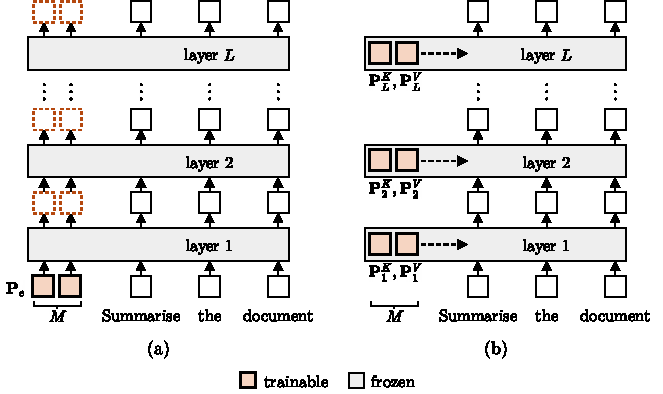
\includegraphics{../diagrams/figures/background/prompt_vs_prefix.pdf}
  \caption{Where the trainable parameters enter a frozen LLM. (a)~Prompt tuning: $M$ learned vectors $\mathbf{P}_e$ are prepended to the input embeddings and processed by the frozen layers like tokens; the dashed outlines mark the hidden states at these positions, computed by the frozen layers. (b)~Prefix tuning: every layer $\ell$ has its own learned keys and values $\mathbf{P}^K_\ell, \mathbf{P}^V_\ell$, which enter the attention of the tokens (dashed arrows); no hidden states are computed at the prefix positions.}
  \label{fig:prompt-prefix}
\end{figure}

%----------------------------------------------------------------------------
\section{Parameter-efficient fine-tuning: LoRA}
\label{sec:lora}
%----------------------------------------------------------------------------

Fine-tuning adapts a pre-trained language model using examples of a desired task or output style~\cite{hu2022lora}. Through further training, the model learns patterns in these examples, such as how to perform the task, structure its output and use the appropriate terminology. However, matching the training examples does not guarantee that its outputs are factually correct or that it will generalise to unfamiliar inputs.

Full fine-tuning updates all model parameters, which is expensive for models with billions of parameters~\cite{hu2022lora}. Parameter-efficient fine-tuning reduces this cost by updating only a small subset of the parameters or by introducing a small number of additional trainable parameters. Soft prompts (\autoref{sec:soft-prompting}) are one such approach: they add learned vectors at the input or in the attention of every layer.

Low-rank adaptation (LoRA)~\cite{hu2022lora} is another. It is based on the hypothesis that the change in the weights during adaptation has a low ``intrinsic rank''. LoRA keeps a pre-trained weight matrix $\mathbf{W}_0 \in \mathbb{R}^{d_{\text{out}} \times d_{\text{in}}}$ frozen and represents its update as the product of two trainable matrices, $\Delta\mathbf{W} = \mathbf{B}\mathbf{A}$, where $\mathbf{B} \in \mathbb{R}^{d_{\text{out}} \times r}$, $\mathbf{A} \in \mathbb{R}^{r \times d_{\text{in}}}$ and the rank $r \ll \min(d_{\text{in}}, d_{\text{out}})$~\cite{hu2022lora}. Both terms are applied to the same input $\mathbf{x}$, and their outputs are summed~\cite{hu2022lora}:
\begin{align}
  \mathbf{h} = \mathbf{W}_0 \mathbf{x} + \frac{\alpha}{r} \mathbf{B}\mathbf{A} \mathbf{x}.
  \label{eq:lora}
\end{align}
Here, $r$ controls the rank of the update and $\alpha$ is a constant that scales its contribution. $\mathbf{A}$ is initialised with random Gaussian values and $\mathbf{B}$ with zeros, so $\Delta\mathbf{W} = \mathbf{0}$ at the beginning of training~\cite{hu2022lora}. The LoRA update therefore initially leaves the model's output unchanged. One adapted matrix adds $r(d_{\text{in}} + d_{\text{out}})$ trainable parameters, instead of the $d_{\text{in}} d_{\text{out}}$ parameters of the full matrix. The smaller parameter count restricts the possible update to each adapted matrix to rank at most $r$.

In principle, LoRA can be applied to any weight matrix of a network. The original experiments adapted only the projection matrices of self-attention; on GPT-3, with the same number of trainable parameters, adapting the query and value projections together gave the best overall results~\cite{hu2022lora}. After training, the update can be added to the frozen weights, $\mathbf{W} = \mathbf{W}_0 + \frac{\alpha}{r}\mathbf{B}\mathbf{A}$, and inference proceeds as usual, with no additional latency compared with a fully fine-tuned model~\cite{hu2022lora}.

%----------------------------------------------------------------------------
\section{Evaluating generated text}
\label{sec:evaluation}
%----------------------------------------------------------------------------

\subsection{Overlap and embedding metrics}
\label{sec:overlap-metrics}

A common approach to automatic evaluation compares generated text with a human-written reference. ROUGE~\cite{lin2004rouge}, introduced for the evaluation of summaries, counts the overlapping units, such as n-grams and word sequences, between a candidate text and the reference. ROUGE-N is an n-gram recall: the number of n-grams of the reference that also occur in the candidate, divided by the number of n-grams in the reference~\cite{lin2004rouge}. ROUGE-1 and ROUGE-2 therefore measure shared words and shared pairs of consecutive words. The precision is computed in the same way, relative to the n-grams of the candidate, and the F1 score is the harmonic mean of the two. ROUGE-L is based on the longest common subsequence of the two texts, which credits words that appear in the same order without requiring them to be consecutive; the length of this subsequence, divided by the lengths of the reference and of the candidate, gives a recall and a precision, which are combined into an F-measure~\cite{lin2004rouge}.

ROUGE measures lexical overlap and can give little credit to paraphrases that use different wording. BERTScore~\cite{zhang2020bertscore} instead compares contextual token embeddings, computed by a pre-trained Transformer encoder. Each token is matched greedily to the most similar token of the other text by cosine similarity~\cite{zhang2020bertscore}, so the matches are not one-to-one: several tokens can be matched to the same token. The method optionally weights tokens by their importance~\cite{zhang2020bertscore}; in the unweighted version, with $\mathbf{u}_1, \dots, \mathbf{u}_k$ the normalised embeddings of the reference tokens and $\hat{\mathbf{u}}_1, \dots, \hat{\mathbf{u}}_l$ those of the candidate, the recall, the precision and the F1 score are
\begin{align}
  R = \frac{1}{k} \sum_{i=1}^{k} \max_{j} \mathbf{u}_i^\top \hat{\mathbf{u}}_j, \qquad
  P = \frac{1}{l} \sum_{j=1}^{l} \max_{i} \mathbf{u}_i^\top \hat{\mathbf{u}}_j, \qquad
  F = \frac{2PR}{P + R}.
  \label{eq:bertscore}
\end{align}
In practice, the scores fall in a narrower range than the $[-1, 1]$ of cosine similarity. The authors therefore propose an optional linear rescaling with respect to an empirical baseline, the average score of random sentence pairs, which makes the scores easier to read without changing how they rank systems~\cite{zhang2020bertscore}.

Agreement with human judgement is the usual test of such metrics. In a study of end-to-end natural language generation systems, word-overlap metrics, including ROUGE, only weakly reflected human ratings of individual outputs and were particularly weak at distinguishing outputs of medium and good quality, although they were more reliable at the level of whole systems~\cite{novikova2017why}.

\subsection{LLM-as-a-judge}
\label{sec:llm-judge}

Human evaluation can assess qualities that similarity metrics capture poorly, but it is costly. LLM-based evaluation offers a more scalable way to assess texts against specified criteria, although its judgements also require validation. An LLM judge can compare two candidate texts or assign a score to a single candidate; in either case, it can also be given a reference text to guide its judgement~\cite{zheng2023judging}. Comparing every pair of systems requires a number of comparisons that grows quadratically with the number of systems, while absolute scores may fluctuate more than pairwise results if the judge model changes~\cite{zheng2023judging}. For numerical grading, the prompt specifies the evaluation criteria and the scale of the scores, and separate criteria can assess different aspects of the text, such as coherence, relevance and factual consistency~\cite{liu2023geval}. On MT-Bench, a set of multi-turn questions, the agreement of GPT-4 with human preferences was comparable to the agreement between human annotators under the reported comparison settings~\cite{zheng2023judging}. This does not show that an LLM judge is equally reliable on other tasks; its reliability has to be checked for the task and the rubric with which it is used.

LLM judges also have systematic biases. Position bias is a preference for an answer because of where it appears in the prompt: in pairwise comparisons, swapping the order of the two answers could reverse the verdict~\cite{wang2024large, zheng2023judging}. A simple countermeasure is to call the judge with both orders and to declare a win only when the same answer is preferred both times~\cite{zheng2023judging}. Verbosity bias is a preference for longer answers, even when they are not as clear, high-quality or accurate as shorter ones~\cite{zheng2023judging}. Self-preference is the tendency of an LLM to score its own outputs higher than texts that human annotators consider of equal quality~\cite{panickssery2024llm}. In summarisation experiments, the evaluated models distinguished their own outputs from those of other models and humans more accurately than chance~\cite{panickssery2024llm}. Experiments that varied self-recognition through fine-tuning also found a correlation between self-recognition and self-preference~\cite{panickssery2024llm}.

%----------------------------------------------------------------------------
\section{Related work: conditioning language models on graphs}
\label{sec:related-work}
%----------------------------------------------------------------------------

G-Retriever~\cite{he2024gretriever} answers questions about graphs whose nodes and edges carry text. To handle graphs that exceed the context window of the LLM, it first selects a smaller subgraph relevant to the question and then generates the answer from this subgraph and the question; \autoref{fig:g-retriever} shows the whole process. The selection starts with retrieval. The text of every node and edge is encoded into an embedding once, in advance, by a frozen pre-trained text encoder. For each question, the question is encoded with the same encoder, and a fixed number of nodes and of edges are retrieved: those whose embeddings have the highest cosine similarity to the embedding of the question~\cite{he2024gretriever}.

Retrieval identifies relevant nodes and edges, but these may be disconnected. G-Retriever therefore constructs a connected subgraph that balances relevance against size. The retrieved nodes and edges receive rewards, called prizes, according to their similarity to the question, while including an edge in the subgraph incurs a fixed cost. G-Retriever seeks a connected subgraph whose total prize minus total edge cost is high, a variant of the prize-collecting Steiner tree problem~\cite{he2024gretriever}. Intermediate nodes without a prize can therefore be included when they connect useful information, like the node in the middle of the selected subgraph in \autoref{fig:g-retriever}.

\begin{figure}[!ht]
  \centering
  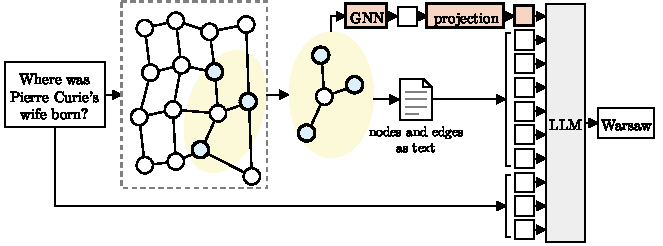
\includegraphics[width=\textwidth]{../diagrams/figures/background/g_retriever.pdf}
  \caption{The G-Retriever pipeline for an illustrative question. In a larger graph, the nodes most similar to the question (blue) are selected, and a connected subgraph is constructed from them (yellow); here it also contains a node that was not selected. A GNN encodes the subgraph into one vector, which a projection maps to a soft prompt. The LLM receives the soft prompt, the nodes and edges of the subgraph written as text, and the question, in this order (from top to bottom), and generates the answer. Trainable components are shown in red, frozen ones in grey.}
  \label{fig:g-retriever}
\end{figure}

To give the LLM a compact summary of the subgraph, G-Retriever encodes it with a GNN. The GNN receives the selected subgraph, that is, its nodes and the connections between them. The input feature of each node is the text embedding computed for it during retrieval~\cite{he2023gretrievercode}. The GNN computes a representation for every node; as in message passing (\autoref{sec:message-passing}), each node representation incorporates information from the connected nodes. Mean pooling, the element-wise average of these node representations, then combines them into one vector for the whole subgraph~\cite{he2024gretriever}.

The graph encoder and the LLM represent information in different vector spaces. A projection network, a small multilayer perceptron, therefore maps the graph vector into the input embedding space of the LLM~\cite{he2024gretriever}. The resulting embedding occupies one additional input position before the embeddings of the rest of the input and acts as a soft prompt (\autoref{sec:soft-prompts}); it is computed from the graph, rather than obtained from the embedding of a vocabulary token. The selected nodes and edges are also listed as text, including their textual attributes. This description and the question form the ordinary textual part of the prompt~\cite{he2024gretriever}. The input of the LLM therefore consists of the soft prompt, followed by the embeddings of the subgraph text and then of the question: the LLM receives both a learned summary of the subgraph and readable text about the same subgraph.

Training uses examples that pair a question and its graph with the expected answer. The loss on the answer tokens is backpropagated through the LLM to the soft prompt, and from there to the projection network and the GNN, which are the only components updated in the main configuration~\cite{he2024gretriever}. The LLM, Llama-2-7B, is frozen: its parameters are not updated, but gradients still pass through it to the trainable components. A further configuration also fine-tuned the LLM with LoRA (\autoref{sec:lora})~\cite{he2024gretriever}.

Experiments in the original paper indicate why the subgraph is given in both forms. In an ablation study on knowledge graph question answering, removing the textual subgraph, so that the LLM received only the soft prompt and the question, lowered the share of correctly answered questions. Replacing the GNN with learned soft prompt vectors that do not depend on the graph lowered it as well~\cite{he2024gretriever}. The authors interpret this as the two representations complementing each other.

A second comparison concerns hallucination. A baseline in which a frozen LLM received a graph only as a soft prompt computed by a trainable GNN often referred, in its answers, to nodes and edges that do not exist in the graph; in a manual check of answers about scene graphs, G-Retriever referred to existing nodes and edges considerably more often~\cite{he2024gretriever}. The authors attribute the errors of the baseline to the difficulty of recalling the structure of an entire graph from a single graph embedding. Since the baseline also did not use retrieval, this comparison does not isolate the effect of the textual input.

While G-Retriever answers questions about a graph, this thesis generates a target node's own text from information about its neighbours. Both approaches use a learned graph representation to guide a language model. G-Retriever adds this representation as a single soft prompt at the input, whereas the method in this thesis produces key and value prefixes for every Transformer layer (\autoref{sec:prefix-tuning}). G-Retriever also supplies the selected subgraph as text, whereas this thesis supplies neighbourhood information only through continuous representations, alongside a fixed textual instruction. Both this thesis and the ablation without textual input require the language model to use a continuous graph representation without directly reading the neighbourhood text. However, the different tasks and conditioning mechanisms mean that the ablation result does not establish how well this approach will work for node-text generation.
